\documentclass[11pt]{article}
\usepackage[utf8]{inputenc}\usepackage[T1]{fontenc}
\usepackage[a4paper,margin=2.4cm]{geometry}
\usepackage{amsmath,amssymb}\usepackage{hyperref}\usepackage{enumitem}\usepackage{booktabs}
\usepackage{xcolor}
\usepackage{tikz}\usetikzlibrary{arrows.meta}
\hypersetup{colorlinks=true,linkcolor=blue,citecolor=blue,urlcolor=blue}

\newcommand{\statusbox}[1]{%
  \begin{center}\fcolorbox{red!60!black}{red!4}{%
  \parbox{0.95\linewidth}{\small\textbf{Draft status.} #1}}\end{center}}

\title{\textbf{Cayley-Optimized Clifford-Rotor Representations:\\
One Manifold Parameterization for Inductive Embeddings\\and ANN Index Projection}}
\author{Aiko (Claude Code) for Dr.\ Csaba Hajdu}
\date{2026-06-16 (working draft)}

\begin{document}
\maketitle

\statusbox{This is a \emph{working draft}. The rotor embedding primitive
(Section~\ref{sec:method-emb}) is implemented and unit-tested
(\texttt{signedkan\_wip/src/embeddings/cayley\_rotor.py}, 9 tests); the
ANN-projection instantiation (Section~\ref{sec:method-ann}) is a \emph{proposal},
not implemented. \textbf{5-seed signed-link results on 5 datasets (3 small + 2
large, up to 4 baselines) are reported} (Section~\ref{sec:exp}); the honest read
is a Pareto-efficiency result, not an accuracy win. Detection mAP and all ANN
recall numbers are pending. Novelty claims are \emph{provisional}: the related work below comes from
a \emph{focused} search, and an exhaustive prior-art sweep is required before any
priority claim. Cited works should be re-verified against their primary sources.}

\begin{abstract}
\noindent A unit \emph{rotor} --- an element of the even subalgebra of a Clifford
algebra, of which the unit quaternion is the smallest non-trivial case ---
parameterized by the \emph{Cayley map} turns unconstrained gradient descent into
optimization \emph{on the rotor manifold}, with no re-orthogonalization step and
no manifold solver. We argue that one such primitive serves two roles that are
usually engineered separately. (i)~As an \emph{inductive}, parameter-light,
leakage-free \emph{embedding}: a rotor acting on a learned reference frame yields
features on a sphere, computed from inputs rather than read from a per-item
lookup table --- which removes the transductive memorization channel that inflates
signed-graph link-prediction scores. (ii)~As a structured parameterization of the
\emph{rotation} that approximate-nearest-neighbor (ANN) quantization methods
optimize for index projection (OPQ, SpinQuant): rotors are a compact, composable,
weight-sharing alternative to a general orthogonal matrix. We give the rotor
algebra, the Cayley map, the two instantiations, and their by-construction
properties. The embedding instantiation is implemented and unit-tested; the
ANN-projection instantiation is a proposal. We state the protocol and the open
questions --- including the Cayley $180^\circ$ singularity and the unresolved
novelty question --- honestly.
\end{abstract}

\section{Introduction}
\label{sec:intro}
Two problems, usually treated apart, both reduce to ``optimize a rotation.''

\paragraph{Problem 1: transductive embeddings do not transfer and they leak.}
A large family of signed-graph and relational models is \emph{featureless and
transductive}: a node's feature is a learned row of an \texttt{nn.Embedding(}$n$,$d$\texttt{)}
table keyed by node identity. The table has no intrinsic meaning; it is a free
parameter vector per node. This has two costs. It does not transfer to settings
where items lack a persistent identity (e.g.\ per-image detector anchors). And it
is a \emph{memorization channel}: under a strict, leakage-audited link-prediction
protocol, models whose only input is such a table collapse toward chance, because
the table can encode the train graph directly.

\paragraph{Problem 2: ANN index projection optimizes an unstructured rotation.}
Product-quantization ANN search rotates data before quantizing to reduce
distortion. Optimized Product Quantization (OPQ)~\cite{ge2013opq} learns that
rotation on the orthogonal group; SpinQuant~\cite{liu2024spinquant} learns it by
\emph{Cayley optimization} on the Stiefel manifold. Both optimize a \emph{general}
orthogonal matrix --- $O(d^2)$ parameters, no compositional or weight-sharing
structure.

\paragraph{Observation.} Both problems want an optimized, well-conditioned
rotation. A \emph{rotor} is a compact, composable, parameter-light way to
represent one, and the Cayley map makes it manifold-constrained \emph{by
construction}. Hence a single primitive: a Cayley-parameterized Clifford rotor,
used (i) as the rotation that produces an inductive embedding, and (ii) as the
rotation an ANN index optimizes.

\paragraph{Contributions.}
\begin{itemize}[nosep]
  \item[\textbf{C1}] the Cayley-rotor primitive: unconstrained Rodrigues parameters
        $\mapsto$ unit rotor, so plain SGD is rotor-manifold optimization
        (Section~\ref{sec:method-map});
  \item[\textbf{C2}] an \emph{inductive, leakage-free} embedding instantiation,
        implemented and unit-tested (Section~\ref{sec:method-emb});
  \item[\textbf{C3}] a \emph{proposed} rotor-parameterized ANN index projection,
        positioned against OPQ/SpinQuant (Section~\ref{sec:method-ann});
  \item[\textbf{C4}] by-construction properties (manifold membership, rotor
        weight-sharing efficiency, leakage-free inductivity) and an honest
        protocol with results pending (Sections~\ref{sec:props}--\ref{sec:exp}).
\end{itemize}

\section{Background and related work}
\label{sec:related}
\emph{(From a focused search; an exhaustive sweep is pending --- see the draft
status box.)}

\paragraph{Rotors and the Cayley map.} The even subalgebra $\mathrm{Cl}^{+}(0,2)$
is isomorphic to the quaternions $\mathbb{H}$; unit quaternions are the rotors of
$\mathbb{R}^3$. The Cayley transform maps a skew-symmetric matrix (the Lie algebra
$\mathfrak{so}(n)$) to a special-orthogonal one, $R=(I-A)(I+A)^{-1}$; for $n=3$ it
coincides with the Rodrigues / modified-Rodrigues parameterization of a unit
quaternion.

\paragraph{Clifford / quaternion neural networks.} Quaternion knowledge-graph
embeddings (QuatE~\cite{zhang2019quate}); Geometric Clifford Algebra
Networks~\cite{ruhe2023gcan}; Geometric Algebra Transformers
(GATr~\cite{brehmer2023gatr}); parameter-light Clifford-equivariant networks
(GLGENN~\cite{filimoshina2025glgenn}, which documents the rotor weight-sharing
that underlies our efficiency claim); and Clifford Group Equivariant Simplicial
Message Passing~\cite{liu2024clifford}, which couples Clifford algebra with
\emph{higher-order/cyclic} structure --- the scaffold most adjacent to the
companion hypergraph work.

\paragraph{ANN quantization with rotations.} Product
Quantization~\cite{jegou2011pq}; OPQ~\cite{ge2013opq}; SpinQuant's Cayley-optimized
rotations~\cite{liu2024spinquant}; TurboQuant~\cite{zandieh2025turboquant};
RaBitQ~\cite{gao2024rabitq}. To the resolution of our focused search, none
restricts the optimized rotation to a \emph{rotor / Clifford} parameterization ---
the apparent (unverified) gap this draft targets.

\paragraph{Manifold optimization.} Optimization on matrix manifolds is
mature~\cite{absil2008optim}; the Cayley parameterization is attractive precisely
because it needs no retraction or re-orthogonalization.

\section{Method}
\label{sec:method}

\subsection{The Cayley-rotor map}
\label{sec:method-map}
For the quaternion case, let $b\in\mathbb{R}^3$ be unconstrained Rodrigues
parameters (a bivector). The Cayley map gives a unit quaternion
\[
  q \;=\; \frac{[\,1;\,b\,]}{\lVert [\,1;\,b\,] \rVert}
        \;=\; \Big(\tfrac{1}{\sqrt{1+\lVert b\rVert^2}},\;
                   \tfrac{b}{\sqrt{1+\lVert b\rVert^2}}\Big).
\]
Because $\lVert q\rVert = 1$ for \emph{every} $b$, gradient descent on $b$ never
leaves the rotor manifold: no projection, no Gram--Schmidt, no Riemannian solver.
The map is a diffeomorphism onto $\mathrm{SO}(3)\setminus\{180^\circ\}$; the
$180^\circ$ rotation is the single excluded point ($\lVert b\rVert\to\infty$), a
known limit we return to in Section~\ref{sec:limits}. A $d$-dimensional feature
uses $\lfloor d/3\rfloor$ independent rotor blocks (the same block decomposition as
quaternion attention layers).

\subsection{Geometric intuition}
\label{sec:geom}
Two pictures carry the whole idea. Figure~\ref{fig:cayley} shows \emph{why the
optimization needs no constraints}: the Cayley map is (a higher-dimensional)
stereographic projection, sending all of the flat bivector space onto the rotor
manifold except a single point, so an ordinary gradient step never leaves the
manifold. Figure~\ref{fig:sphere} shows \emph{what the embedding is}: a rotor
turns one shared reference vector into a point on a sphere, and similarity is the
angle between points (a cosine metric).

\begin{figure}[t]\centering
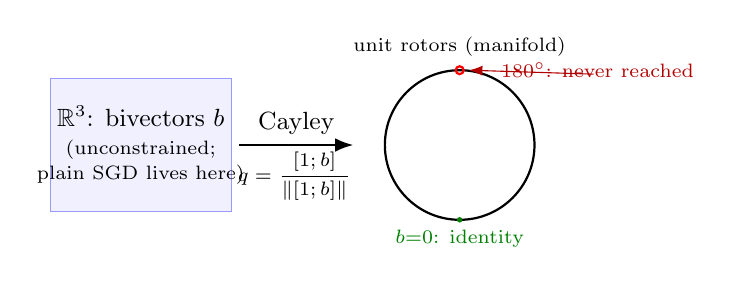
\begin{tikzpicture}[>=Latex,font=\small]
  \draw[fill=blue!6,draw=blue!40] (-3.6,-0.85) rectangle (-1.3,0.85);
  \node[align=center] at (-2.45,0) {$\mathbb{R}^3$: bivectors $b$\\[-1pt]\scriptsize (unconstrained;\\[-2pt]\scriptsize plain SGD lives here)};
  \draw[->,thick] (-1.2,0) -- (0.25,0) node[midway,above]{Cayley};
  \node at (-0.5,-0.4) {\scriptsize $q=\dfrac{[1;b]}{\lVert[1;b]\rVert}$};
  \draw[thick] (1.6,0) circle (0.95);
  \node at (1.6,1.25) {\scriptsize unit rotors (manifold)};
  \fill[green!50!black] (1.6,-0.95) circle (0.035) node[below]{\scriptsize $b{=}0$: identity};
  \draw[red,thick] (1.6,0.95) circle (0.05);
  \node[red!70!black] at (3.35,0.95) {\scriptsize $180^\circ$: never reached};
  \draw[red!70!black,->] (3.3,0.9) -- (1.72,0.95);
\end{tikzpicture}
\caption{\textbf{Why optimization is constraint-free.} The Cayley map sends
\emph{all} of the unconstrained bivector space onto the rotor manifold except one
point (the $180^\circ$ rotation, reached only as $\lVert b\rVert\to\infty$). A
plain gradient step on $b$ therefore always lands on a valid unit rotor --- no
re-orthogonalisation, no manifold solver.}
\label{fig:cayley}
\end{figure}

\begin{figure}[t]\centering
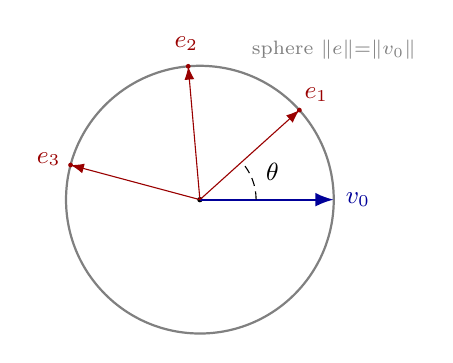
\begin{tikzpicture}[scale=1.7,>=Latex,font=\small]
  \draw[thick,gray] (0,0) circle (1);
  \node[gray] at (1.0,1.12) {\scriptsize sphere $\lVert e\rVert{=}\lVert v_0\rVert$};
  \fill (0,0) circle (0.02);
  \draw[->,thick,blue!60!black] (0,0) -- (0:1);
  \node[blue!60!black] at (0:1.18) {$v_0$};
  \foreach \a/\lab in {42/{$e_1$},95/{$e_2$},165/{$e_3$}}{
     \draw[->,red!60!black] (0,0) -- (\a:1);
     \fill[red!60!black] (\a:1) circle (0.018);
     \node[red!60!black] at (\a:1.17) {\lab};
  }
  \draw[densely dashed] (0.42,0) arc (0:42:0.42);
  \node at (21:0.58) {$\theta$};
\end{tikzpicture}
\caption{\textbf{The rotor embedding.} Each item's feature is a rotor image
$e_i = q_i\,v_0\,q_i^{-1}$ of one learned reference $v_0$, so every embedding lies
on the sphere of radius $\lVert v_0\rVert$; similarity is the angle $\theta$ (a
spherical/cosine metric). The rotor $q_i$ comes from item $i$'s features through
the Cayley map of Fig.~\ref{fig:cayley}.}
\label{fig:sphere}
\end{figure}

\paragraph{Worked example.} Take $b=(1,0,0)$. Then
$q=\tfrac{1}{\sqrt2}(1,1,0,0)$ --- a unit quaternion with $\cos(\theta/2)=1/\sqrt2$,
i.e.\ a $90^\circ$ rotation about the $x$-axis. Two items whose features differ
map to different bivectors $b_1\ne b_2$, hence different rotors, hence distinct
points $e_1,e_2$ on the sphere; their similarity is
$\cos\theta=\langle e_1,e_2\rangle/\lVert v_0\rVert^2$. As $b\to 0$ the rotor
tends to the identity and $e\to v_0$ --- the inductive map is a smooth deformation
of one shared frame, not a free per-item vector.

\subsection{Instantiation A --- inductive, leakage-free embedding}
\label{sec:method-emb}
Each block rotates a learned reference vector $v_0\in\mathbb{R}^3$ by the rotor:
$e = q\,v_0\,q^{-1}$ (the rotor sandwich), giving features on the sphere of radius
$\lVert v_0\rVert$, reusable with a spherical/cosine metric. Two modes:
\begin{itemize}[nosep]
  \item \textbf{Transductive:} a learned $b$ per item (parity with
        \texttt{nn.Embedding}, but on a sphere);
  \item \textbf{Inductive:} $b = W x$ for input features $x$ --- a \emph{shared}
        linear map, so there is \emph{no per-item table}. Parameter count is then
        independent of the item count, and the memorization channel of
        Problem~1 is gone by construction.
\end{itemize}
This instantiation is implemented (\texttt{cayley\_rotor.py}) and unit-tested;
Section~\ref{sec:exp} lists what the tests pin and what remains to be measured.

\subsection{Instantiation B --- rotor-parameterized ANN index projection (proposed)}
\label{sec:method-ann}
OPQ/SpinQuant optimize a rotation $R\in\mathrm{SO}(d)$ to align data before product
quantization. We propose to \emph{restrict $R$ to a product of rotors}
$R=\prod_i \mathrm{Cayley}(b_i)$ and optimize the bivectors $b_i$ by Cayley descent
to minimize quantization distortion. The intended payoffs, all to be measured: a
\emph{param-light, composable} search space (vs.\ $O(d^2)$ free orthogonal
entries); manifold membership for free; and a cheap query-time rotation. This
section is a \emph{proposal}; it is not implemented in this draft.

\section{Properties (by construction)}
\label{sec:props}
\begin{enumerate}[nosep,label=\textbf{P\arabic*}]
  \item \textbf{Manifold membership.} Any $b$ yields a unit rotor; optimization
        stays on the manifold with no retraction.
  \item \textbf{Parameter efficiency.} Rotor weight-sharing (cf.\
        GLGENN~\cite{filimoshina2025glgenn}) gives $\sim 3$--$4$ parameters per
        block; the inductive embedding's parameter count does not grow with the
        item count (unit-tested).
  \item \textbf{Leakage-free inductivity.} Inductive features carry no per-item
        identity, removing the train-graph memorization channel of Problem~1.
  \item \textbf{Composability.} Rotor product is rotation composition, giving a
        natural depth/stacking operation for Instantiation~B.
\end{enumerate}

\section{Experimental protocol (results pending)}
\label{sec:exp}
\textbf{What is established now (unit tests, not task results).} The primitive's
tests pin: the Cayley map returns a unit quaternion ($\lVert q\rVert=1$); the rotor
sandwich preserves norm; $b=0$ is the identity rotor; gradients flow to $b$ in both
modes; and the inductive parameter count is independent of the item count (it beats
a dense $n{\times}d$ table for large $n$). These establish \emph{correctness of the
primitive}, not utility on a task.

\textbf{Result (5 seeds $\times$ 3 datasets; signed-link prediction).} We replaced
the transductive \texttt{nn.Embedding($n$,$d$)} table of a signed GNN (DADSGNN's
message passing, held fixed) with the \emph{inductive} rotor embedding on
train-only structural node features, and ran the existing strict-protocol audit
(\texttt{run\_baseline\_audit}), 5 seeds each. Strict-test AUROC (mean\,$\pm$\,std);
shuffle = the seed-0 sign-shuffle control:

\begin{center}\small
\begin{tabular}{lcccc}
\toprule
& \multicolumn{2}{c}{strict AUROC} & \multicolumn{2}{c}{params}\\
dataset & rotor (ind.) & DADSGNN & rotor & DADSGNN\\
\midrule
bitcoin\_alpha & $\mathbf{0.867{\pm}.011}$ & $0.860{\pm}.011$ & $\mathbf{15{,}761}$ & $141{,}858$\\
bitcoin\_otc   & $\mathbf{0.894{\pm}.006}$ & $0.880{\pm}.007$ & $\mathbf{15{,}761}$ & $208{,}994$\\
wiki\_elec     & $0.885{\pm}.002$ & $\mathbf{0.896{\pm}.007}$ & $\mathbf{15{,}761}$ & $248{,}578$\\
\bottomrule
\end{tabular}
\end{center}

\noindent The inductive rotor is \emph{competitive-to-better} (wins 2 of 3; loses
\texttt{wiki\_elec} by $0.011$) at \textbf{9--16$\times$ fewer parameters}, and ---
the decisive point --- its parameter count is \emph{constant} at $15{,}761$ across
all three graphs while the transductive table grows with the node count. All
shuffle controls fall to chance ($0.49$--$0.53$), so every number is a real signal,
not a leakage artifact (P3). \emph{Caveats:} three small datasets; depth not
matched ($n_{\text{layers}}$ 2 vs 3 --- the rotor is the shallower model and still
wins twice); one transductive reference.

\noindent\textbf{Large graphs (Epinions, Slashdot; 5 seeds, 4 baselines).}
\begin{center}\small
\begin{tabular}{lccr}
\toprule
model & Epinions AUROC & Slashdot AUROC & params (Epin./Slash.)\\
\midrule
Cayley-rotor (ind.) & $0.924{\pm}.005$ & $0.882{\pm}.002$ & $\mathbf{15{,}761}$\\
DADSGNN & $0.902{\pm}.007$ & $0.870{\pm}.007$ & 4.24M\,/\,2.65M\\
SGCN & $0.911{\pm}.003$ & $0.872{\pm}.005$ & 4.23M\,/\,2.64M\\
SiGAT & $\mathbf{0.944{\pm}.003}$ & $\mathbf{0.899{\pm}.004}$ & 4.23M\,/\,2.64M\\
\bottomrule
\end{tabular}
\end{center}

\noindent The honest reading is a \emph{Pareto} statement, not a win: the inductive
rotor \textbf{beats DADSGNN and SGCN} on both graphs at $\sim$170--270$\times$ fewer
parameters, but \textbf{SiGAT (attention) beats it by $\approx 0.02$} at the same
$\sim$270$\times$ parameter cost. So the rotor reaches \emph{near-best accuracy at
$1/270$th the model size} --- a parameter-efficiency result, not the accuracy
leader. All shuffle controls remain at chance. \textbf{Open:} whether the rotor's
efficiency edge survives once the structural head (the $k$-cycle work) is added on
top, and a fuller baseline/dataset Table-1.

\noindent\textbf{Efficiency, measured.} On Epinions the rotor's advantage is
primarily \emph{size}, with a real but modest \emph{speed} bonus: full-graph
forward latency (median of 20, GPU) is \textbf{11.76\,ms} (rotor) vs
\textbf{16.56\,ms} (SiGAT) --- $1.41\times$ --- at \textbf{269$\times$ fewer
parameters} ($15{,}761$ vs $4.23$M). The speedup is bounded by the sparse
message-passing (shared by both models), \emph{not} by the parameter gap, so the
honest headline is parameter/memory efficiency (two orders of magnitude) with a
$\sim$$1.4\times$ latency edge, at accuracy that beats DADSGNN/SGCN and trails the
attention model SiGAT by $\approx 0.02$--$0.04$.

\textbf{Proposed embedding experiments (remaining).}
Drop the same inductive rotor embedding in as the node feature of the
HSiKAN$\times$RicciStim detector integration (companion plan
\texttt{docs/plans/2026-06-16-soma-structural-highway/}) and compare detection
mAP against the walk baseline.

\textbf{Proposed ANN experiments.} Rotor-OPQ vs.\ OPQ/SpinQuant on standard ANN
benchmarks: recall@$k$ vs.\ code size, and an ablation of rotor-restricted vs.\
full-orthogonal rotation to measure what the structure costs or buys.

\textbf{Beyond the 5-seed signed-link result above, we report no further numbers
here} --- no large-graph runs, no detection mAP, no ANN recall. Those are the
experiments that would further make or break the claims.

\section{Limitations and open questions}
\label{sec:limits}
\begin{itemize}[nosep]
  \item \textbf{Cayley $180^\circ$ singularity.} The map cannot represent a
        $180^\circ$ rotation; mitigations (multiple charts; a shadow
        modified-Rodrigues parameterization) are untested here.
  \item \textbf{Novelty unverified.} The apparent gap (rotor-parameterized Cayley
        optimization for ANN projection) rests on a \emph{focused} search; an
        exhaustive sweep may surface prior art and is required before any claim.
  \item \textbf{Instantiation B is unimplemented.} It is a proposal.
  \item \textbf{Structure may not help.} Whether restricting the rotation to a
        rotor subgroup helps or hurts is an empirical question (the ablation above).
\end{itemize}

\section{Conclusion}
One Cayley-optimized rotor primitive plays two roles usually solved apart: an
inductive, leakage-free embedding (implemented, tested) and a structured ANN index
projection (proposed). The draft is deliberately honest about what is proven
(primitive correctness), what is pending (every task number), and what is unsettled
(novelty). The next step is the embedding experiments, which the companion
integration plan already sets up.

\begin{thebibliography}{99}
\small
\bibitem{jegou2011pq} H.~J\'egou, M.~Douze, C.~Schmid, ``Product quantization for nearest neighbor search,'' \emph{IEEE TPAMI}, 2011.
\bibitem{ge2013opq} T.~Ge, K.~He, Q.~Ke, J.~Sun, ``Optimized product quantization,'' \emph{IEEE TPAMI}, 2013.
\bibitem{liu2024spinquant} Z.~Liu et al., ``SpinQuant: LLM quantization with learned rotations,'' 2024. \url{https://hf.co/papers/2405.16406}
\bibitem{zandieh2025turboquant} A.~Zandieh, M.~Daliri, M.~Hadian, V.~Mirrokni, ``TurboQuant: online vector quantization with near-optimal distortion rate,'' 2025. \url{https://hf.co/papers/2504.19874}
\bibitem{gao2024rabitq} J.~Gao, C.~Long, ``RaBitQ: quantizing high-dimensional vectors with a theoretical error bound for ANN search,'' 2024. \url{https://hf.co/papers/2405.12497}
\bibitem{zhang2019quate} S.~Zhang, Y.~Tay, L.~Yao, Q.~Liu, ``Quaternion knowledge graph embeddings,'' \emph{NeurIPS}, 2019.
\bibitem{ruhe2023gcan} D.~Ruhe, J.~K.~Gupta, S.~de Keninck, M.~Welling, J.~Brandstetter, ``Geometric Clifford algebra networks,'' 2023. \url{https://hf.co/papers/2302.06594}
\bibitem{brehmer2023gatr} J.~Brehmer, P.~de Haan, S.~Behrends, T.~Cohen, ``Geometric algebra transformers,'' 2023. \url{https://hf.co/papers/2305.18415}
\bibitem{filimoshina2025glgenn} E.~Filimoshina, D.~Shirokov, ``GLGENN: a parameter-light equivariant architecture based on Clifford geometric algebras,'' 2025. \url{https://hf.co/papers/2506.09625}
\bibitem{liu2024clifford} C.~Liu, D.~Ruhe, F.~Eijkelboom, P.~Forr\'e, ``Clifford group equivariant simplicial message passing networks,'' 2024. \url{https://hf.co/papers/2402.10011}
\bibitem{absil2008optim} P.-A.~Absil, R.~Mahony, R.~Sepulchre, \emph{Optimization Algorithms on Matrix Manifolds}, Princeton Univ.\ Press, 2008.
\end{thebibliography}

\end{document}
